% ======================================================================

\chapter{Raceline Optimization}
\label{chap:opt}

Lo studio di questa tesi si è concentrato a trovare una soluzione al seguente problema:\
\textit{trovare la raceline globale ottima \emph{\footnotesize -- secondo un criterio scelto --} data una mappa}.
Il criterio di ottimizzazione principale, in questi casi, è il tempo di percorrenza del tracciato, ovvero
il \textit{laptime}.

Le porzioni interessanti di un circuito da gara sono le curve: ne esistono di diversi tipi e altrettanti
modi per affrontarle in base al tipo; trovare una percorso ottimo, in questo senso, è un compito complesso e
il percorso più breve non implica quello col minor tempo per via, appunto, delle curve, che riducono la
velocità media. Dunque una strategia migliore è quella di trovare la traiettoria con le curvature minori,
così da mantenere una velocità più alta nell'affrontarle. Anche questo approccio, tuttavia, non prende in
considerazione una sequenza di curve e la velocità di uscita da una curva. Il percorso ottimo in termini
di tempo, quindi, è un compromesso tra queste due strategie, ovvero quello che minimizza la distanza
percorsa mantenendo alta la velocità nelle curve ed eventualmente anche in uscita da esse.

É bene precisare che la traiettoria generata è ottima \textbf{solo} nel contesto considerato, ovvero
quello di un singolo robot sul tracciato, senza alcun rivale. È da considerare un'operazione preliminare
alla gara, perchè si ha necessità di conoscere la mappa.
Tuttavia non è utile solo nel contesto considerato: la raceline ottima, avendo una visione globale sulla
mappa, può essere sfruttata da un local o behavioural planner come linea guida.

\section{Le curve}
Il fulcro di cui l'ottimizzazione si occupa è come affrontare le curve.\\
Caratteristica principale di una curva è il suo raggio: un raggio maggiore corrisponde a velocità più alte
e viceversa; inoltre, si distinguono il raggio esterno e quello interno e la loro differenza risulta
nell'ampiezza della curva.
Esistono anche caratteristiche di natura tridimensionale, come la variazione dell'altezza e
l'inclinazione, tuttavia non sono state oggetto di studio in questa tesi dal fatto che il contesto di
F1TENTH non include questa variabilità, come accade nelle gare di F1.

In linea generale, una curva può essere suddivisa in quattro sequenze principali: %, come mostrato in figura:%TODO: ref
\begin{enumerate}
	\item Approccio e decelazione
	\item Inizio della curva
	\item Raggiunta dell'apice
	\item Uscita della curva e accelerazione
\end{enumerate}

Anche la traiettoria, dato che segue una curva, può essere definita con un raggio che può essere
costante o variabile dall'inzio della curva fino alla fine.

\begin{figure}[h]
	\begin{center}
		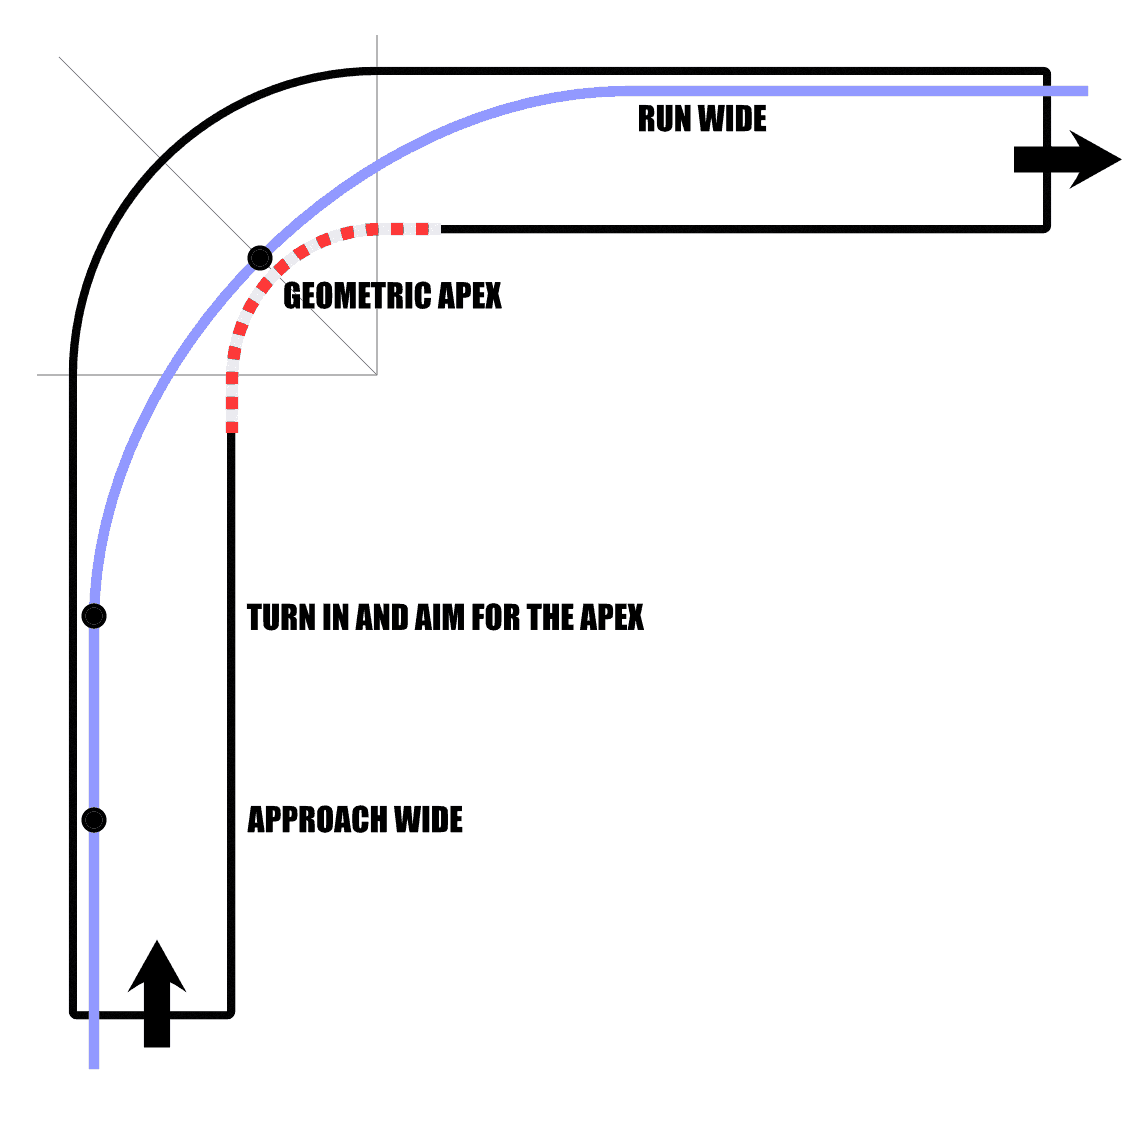
\includegraphics[width=0.65\textwidth]{geometric-apex.png}
	\end{center}
	\caption{Rappresentazione delle fase di una raceline geometrica per una curva a destra}\label{fig:geom-raceline}
\end{figure}

\paragraph{Raceline geometrica}
L'approccio più semplice e immediato per affrontare una curva genera una raceline che prende il
nome di \textit{raceline geometrica}. La strategia prevedere queste sequenze, rappresentate in figura
\ref{fig:geom-raceline}:
\begin{enumerate}
	\item Approccio largo e verso l'esterno del circuito 
	\item Sterzata verso il centro del raggio interno della curva 
	\item Uscita larga e verso l'esterno del circuito
\end{enumerate}
Si tratta, quindi, di una raceline a raggio costante.\\
I principali vantaggi di questo approccio rispetto alla raceline ottima sono la sua semplicità, sia in
termini di esecuzione sia in termini di computazione, e la possibilità di mantenere un'alta velocità
durante la curva. Tuttavia, la raceline geometrica ha importanti svantaggi quali una decelazione
prematura all'entrata della curva, una accelerazione ritardata all'uscita e la possibilità di essere in
uno stato svantaggiato per affrontare la prossima curva, nel caso di curve in sequenza.

Dunque, la raceline ottimale non dovrebbe tener conto solamente della singola curva ma eventualmente
anche di quelle successive: per estensione, quindi, deve essere considerato tutto il circuito.

\paragraph{Raceline ottimale}
Al contrario della raceline geometrica, non è possibile definire a priori le sequenze da seguire come
fatto in precedenza, proprio perchè dipende dalle caratteristiche della curva.
Riprendendo come esempio la curva in figura \ref{fig:geom-raceline}, la raceline ottimale, ovvero quella
che riesce ad eseguire la curva nel minor tempo possibile, tarda il più possibile l'inizio della curva
per mantenere più velocità all'entrata, decelera più velocemente e ha una virata più stretta e con un
apice più distante da quello geometrico, così facendo si ha la possibilità di aver più tempo per
accelerare di nuovo all'uscita della curva con la possibità di mantenere una traiettoria più centrata
rispetto al circuito.

In figura \ref{fig:cmp-lines} vi è una comparazione grafica tra le due raceline.\\
La raceline ottima, inoltre, adegua la traiettoria di uscita in base alla curva successiva, se presente,
in modo tale da affrontarla anch'essa nel modo ottimale. Si nota la distinzione in figura
\ref{fig:cmp-opt-lines}.

\begin{figure}[H]
	\begin{minipage}[c]{0.45\textwidth}
		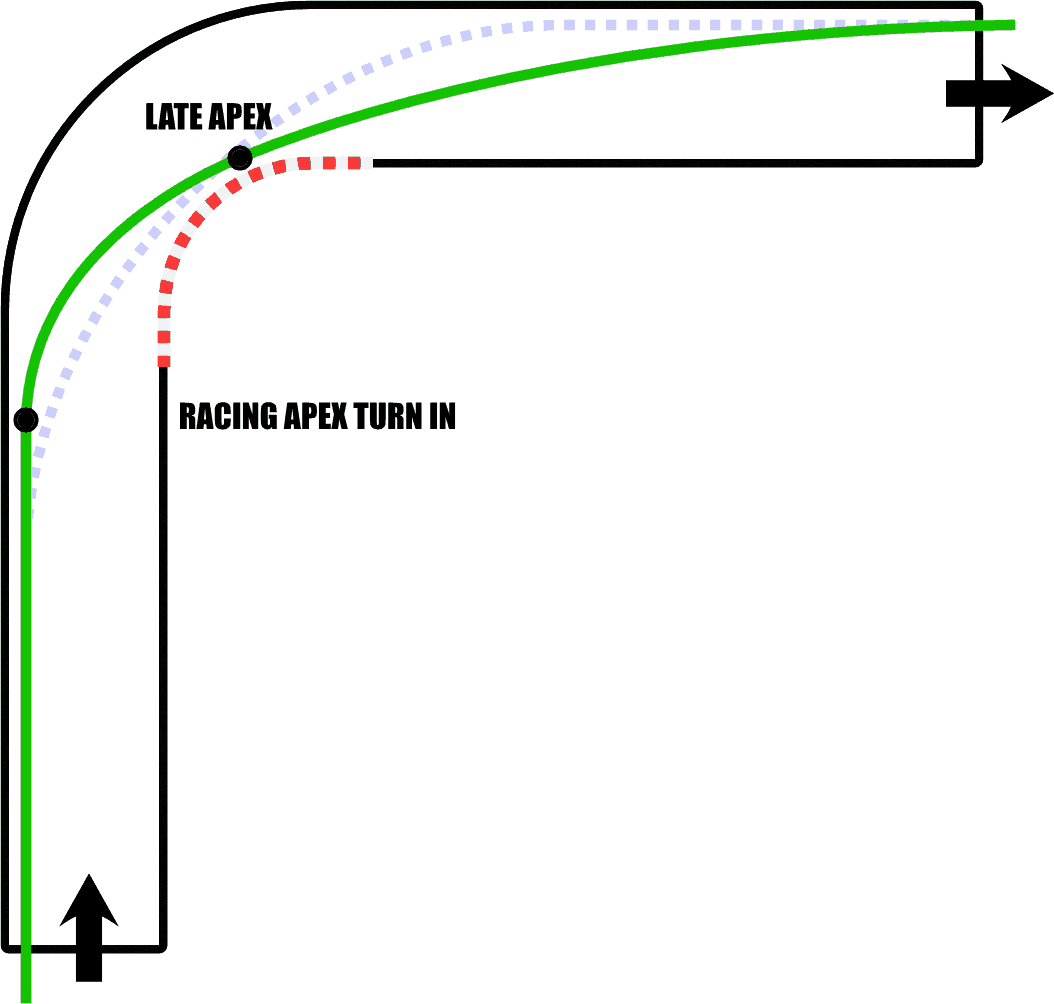
\includegraphics[width=0.80\textwidth]{comparing-lines.png}
		\caption{Comparazione tra raceline ottimale, in verde, e raceline geometrica, in blu tratteggiato}\label{fig:cmp-lines}
	\end{minipage}\hfill
	\begin{minipage}[c]{0.45\textwidth}
		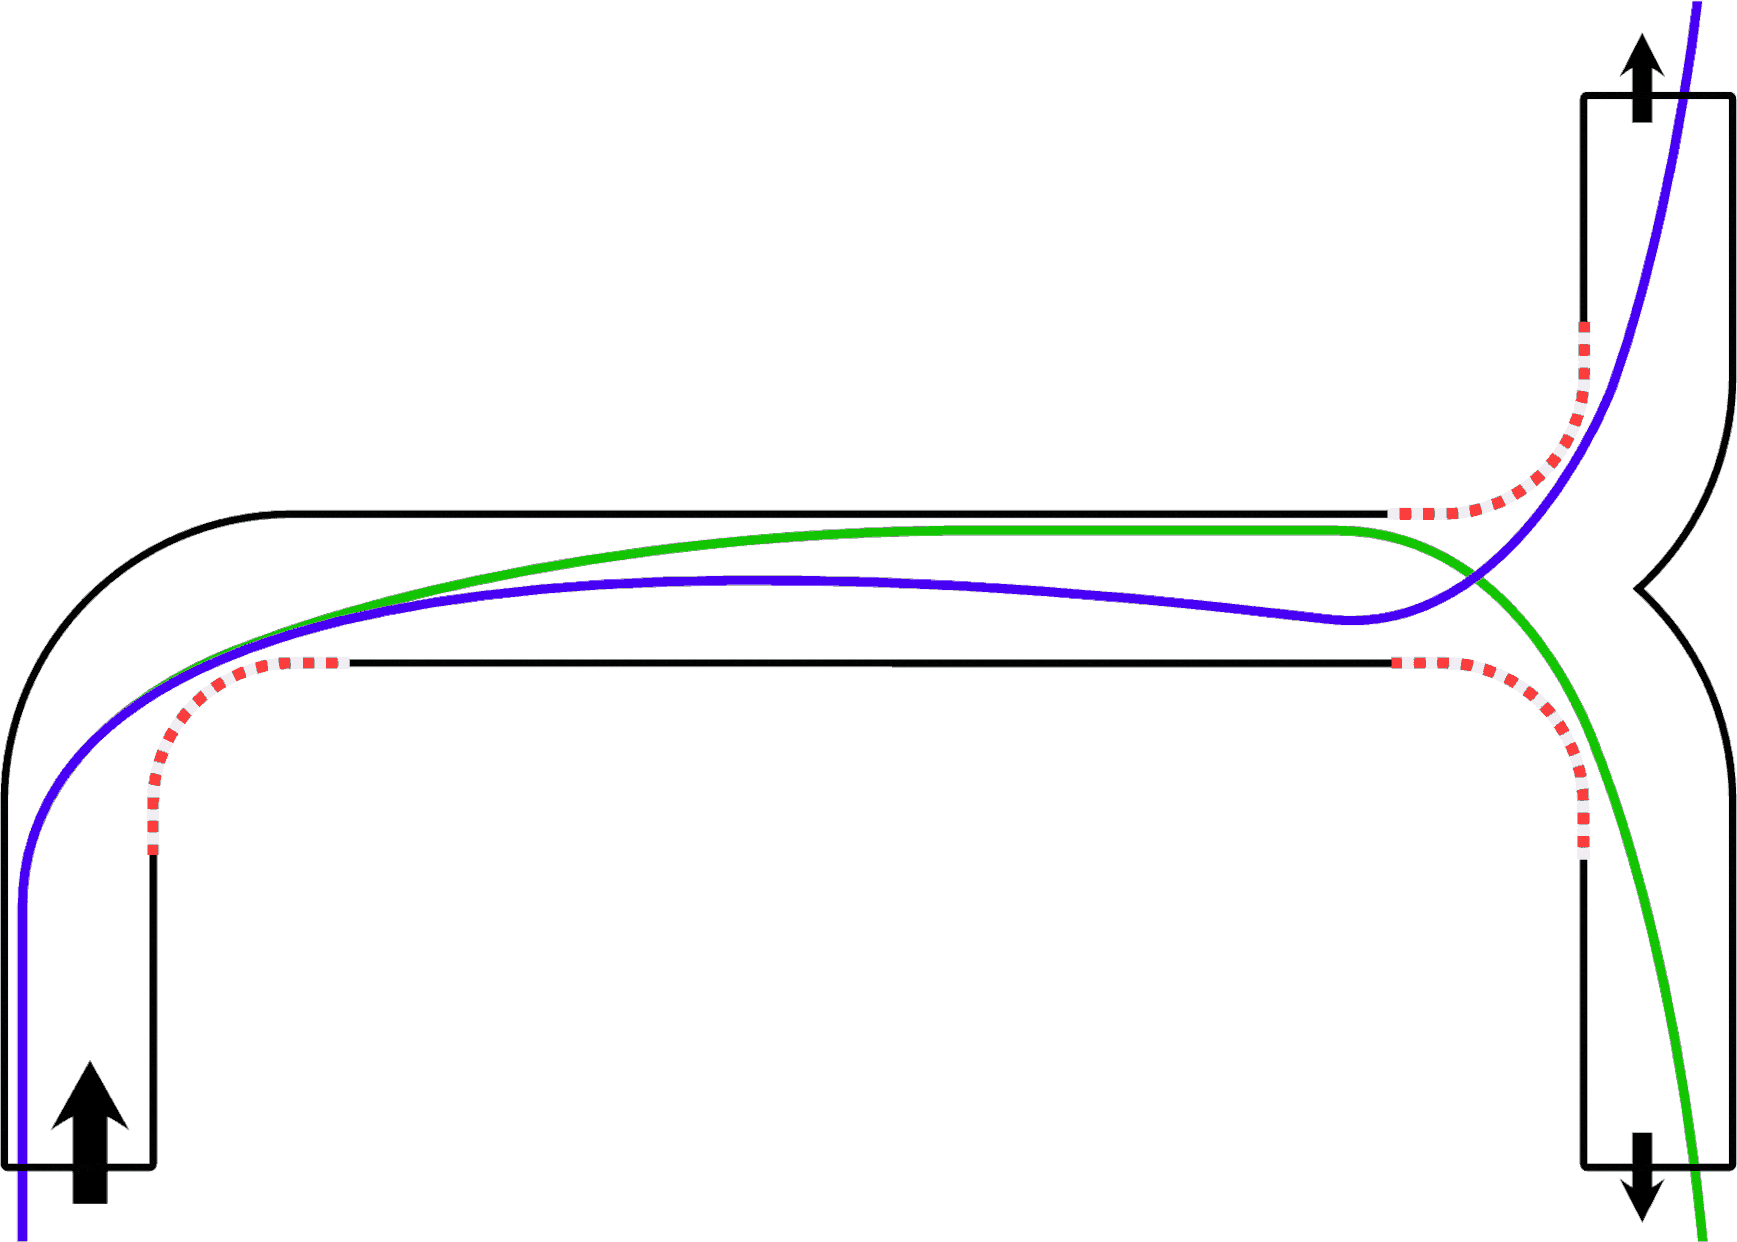
\includegraphics[width=1\textwidth]{multiple-corners.png}
		\caption{Confronto tra raceline ottime con due curve distinte in sequenza}\label{fig:cmp-opt-lines}
	\end{minipage}
\end{figure}


% ========= Processo di Generazione ====================================
% Il lavoro è stato basato su questa repo \url{https://github.com/CL2-UWaterloo/Raceline-Optimization}.
\section{Processo di generazione}
% fonti: L22 Raceline-Optimization slide

Di seguito si presentano alcune definizioni più formali dei termini utilizzati precedentemente e il
processo di generazione del percorso ottimo secondo un certo criterio.

\bigskip
\noindent In questa tesi sono state analizzate tre strategie differenti:
\begin{itemize}
	\setlength\itemsep{0em}
	\item Percorso più breve  -- \textit{shortest path}
	\item Curvatura minima -- \textit{minimum curvature}
	\item Tempo minimo -- \textit{minimum time}
\end{itemize}

\noindent Il problema in questione è un problema di ricerca su due variabili: il percorso effettivo sulla mappa e
la velocità da mantenere per ogni punto del percorso. Queste due variabili assieme definiscono la
\textit{traiettoria} o \textit{raceline}, in inglese.\\
I vincoli applicati alla ricerca sono due: i limiti dinamici del veicolo, per esempio quanta forza G il
veicolo riesce a sostenere in sterzata, e gli ostacoli statici, rappresentati dai bordi del circuito.

\bigskip
\noindent Il problema viene suddiviso in due sottoproblemi, ovvero risolvere singolarmente la ricerca sulle due
variabili in gioco. Si distinguono quindi, in sequenza:
\begin{enumerate}
\setlength\itemsep{0em}
\item Generazione del percorso secondo i vincoli desiderati -- \textit{path planning}
\item Calcolo della velocità sul percorso generato -- \textit{velocity planning}
\end{enumerate}
In particolare, il path planning viene modellato come un problema di programmazione quadratica geometrica
(Geometric QP), che ha i vantaggi di richiedere pochi parametri e di essere computazionalmente veloce;
esistono anche altri tipi di algortimi di ottimizzazione basati su evoluzione, come CMA-ES. Il velocity
planning può essere risolto con algortimi a stato quasi-stazionario come l'algoritmo forward-backward. Un
ulteriore metodo per il velocity planning per il tempo più breve è descritto in \textit{"Minimum-time
speed optimisation over a fixed path"} \cite{lipp2014minimum}.

Per quanto riguarda la terza strategia, i due sottoproblemi possono anche essere risolti contemporaneamente
usando algoritmi di controllo ottimale, questi hanno la possibilità di includere ulteriori vincoli come
per esempio limitazioni al consumo di energia.

\subsection{Definizioni formali}
\label{sub:formal-def}
% section a parte?
\paragraph{Definizione di spline \cite{olausson2021optimal} \cite{globalplanning-lec}}
\label{par:spline-def}
Un percorso, per poter essere computato da una macchina, deve necessariamente essere discretizzato in
punti, detti \textit{samples}.
Tuttavia è necessaria una descrizione matematica del tracciato: questa viene risolta con l'uso delle
\textit{spline}. Una spline è una funzione definita a pezzi da un'insieme di polinomi dello stesso grado
il cui scopo, in questo contesto, è quello di interpolare dei punti, ovvero i samples, in modo tale che
la funzione sia continua fino ad un dato ordine.

Il problema richiedere alcuni vincoli per le spline. Per rappresentare un percorso, che deve essere
seguito da un'auto, è necessario che la spline sia continua e derivabile almeno fino al secondo grado per
le seguenti motivazioni:
\begin{itemize}
	\item è necessario che la direzione dell'auto alla fine di un polinomio sia uguale all'inizio di
		quello successivo -- la derivata prima garantisce questo 
	\item è necessario che la curvatura alla fine di un polinomio sia uguale all'inizio di quello
		successivo -- la derivata seconda garantisce questo
\end{itemize}
È sufficiente, quindi, che la spline si almeno di grado tre, così da garantire la calcolabilità della
prima e della seconda derivata per ogni punto.
Un esempio dell'uso di una spline per interpolare dei punti è mostrato in figura \ref{fig:spline}

\begin{figure}[H]
	\begin{center}
		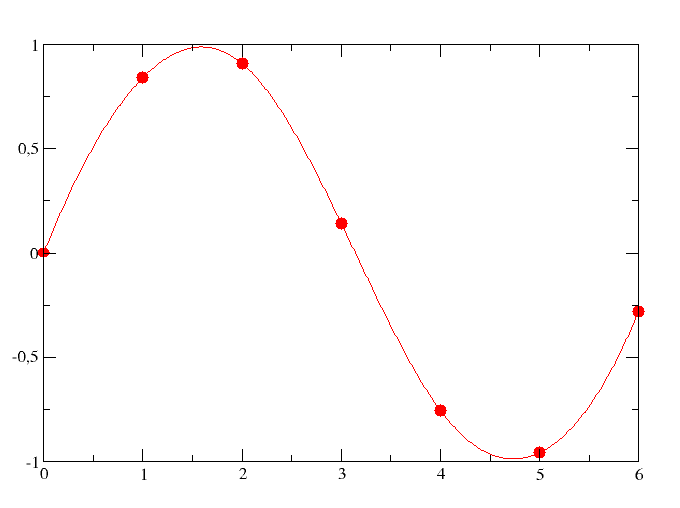
\includegraphics[width=0.55\textwidth]{spline-interpol.png}
	\end{center}
	\caption{Esempio di interpolazione spline}\label{fig:spline}
\end{figure}

\paragraph{Definizione di centerline}
\label{par:centerline}
La centerline o reference line è il percorso sul circuito preso in considerazione che è equidistante dai
bordi dello stesso. Viene discretizzata in punti di egual distanza tra loro e si registrano le distanze
ai bordi destro e sinistro così da formare una line immaginaria, ortogonale alla refence line, che unisce
i due punti. L'immagine \ref{fig:centerline-ex} ne mostra un esempio grafico.

La linea centrale di riferimento è necessaria agli algortimi di ottimizzazione come punto di partenza per
trovare la soluzione ottima.
La distanza dei samples è un parametro dell'algoritmo e deve essere decisa in base al caso d'uso.

\begin{figure}[h]
	\begin{center}
		%TODO: da cambiare? troppo sgranato?
		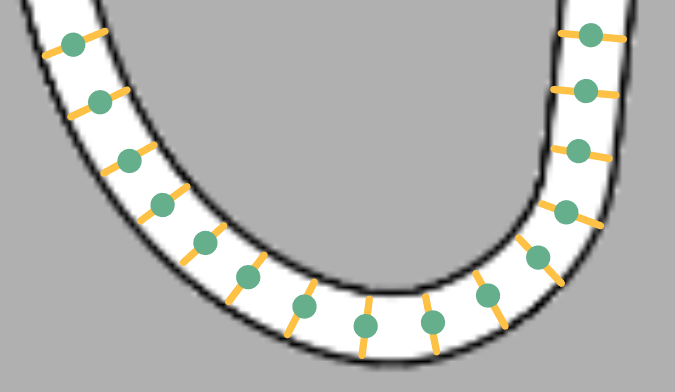
\includegraphics[width=0.65\textwidth]{centerline-ex.png}
	\end{center}
	\caption{La figura mostra la rappresentazione discreta della centerline (i punti verdi) e le linee
	immaginarie (quelle gialle) che uniscono, ortonogonalmente rispetto alla centerline, i bordi
	del circuito}\label{fig:centerline-ex}
\end{figure}

\paragraph{Definizione di raceline}
% Anche la raceline, come la \ref[par:centerline]{centerline}, deve essere discretizzata.\\
I samples della raceline vengono calcolati a partire da quelli delle centerline muovendoli sulla linea
che unisce i due tracciati. Formalmente:
\[
	\overrightarrow{r_i} = \overrightarrow{p_i} + \alpha_i \overrightarrow{n_i}
\]
dove il sample $i$ della raceline $r$, descritto dal vettore $\overrightarrow{r_i}$, viene traslato di un
fattore $a_i$ lungo il vettore $\overrightarrow{n_i}$, ovvero la linea che unisce i bordi del circuito.
La figura \ref{fig:raceline-def} rappresenta graficamente questo processo.

\begin{figure}[h]
	\begin{center}
		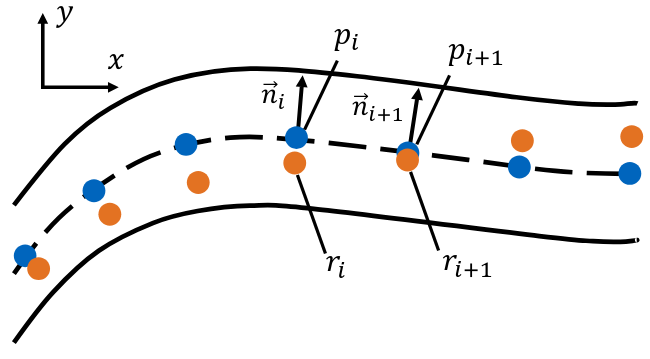
\includegraphics[width=0.75\textwidth]{raceline-def.png}
	\end{center}
	\caption{Rappresentazione grafica della raceline, dove i punti blu rappresentano i samples della
	centerline, mentre quelli arancioni sono quelli della raceline, traslati di un certo fattore lungo i
	vettori $n$ corrispondenti}
	\label{fig:raceline-def}
\end{figure}

È necessario, inoltre, imporre un vincolo sul fattore $a$ in modo tale che non venga prodotto un sample
al di fuori del circuito o che non permetta al robot di passare perchè troppo vicino ai bordi.
Formalmente:
\begin{equation}
	a_i \in [ -w_{tr\_left, i} + \frac{w_{veh}}{2}, w_{tr\_right, i} - \frac{w_{veh}}{2}]
	\label{eq:a_constr}
\end{equation}
dunque, dato un indice $i$, il fattore $a$ deve rientrare nel range definito tra la distanza del circuito
a sinistra $w_{tr\_left}$ del sample della centerline dello stesso indice e la distanza a destra
$w_{tr\_right}$ aggiustato per la larghezza del veicolo $w_{veh}$.

\subsection{Modelli formali}
Ora verranno esaminate più in dettaglio il modello dei problemi di QP
geometrico per le strategie di percorso più breve e minor curvatura.

La programmazione quadratica è un processo che risolve problemi di ottimizzazione matematica descritti da
funzioni quadratiche. L'obiettivo è quello di trovare un vettore che minimizzi o massimizzi il valore di
una funzione obiettivo preservando contemporaneamente dei vincoli, descritti da diseguazioni.

\paragraph{Percorso più breve}\cite{race-model}\cite{globalplanning-lec}
Il modello in questione deve descrivere il percorso più breve, ovvero che abbia la distanza minore tra i
samples. Un sample della raceline viene formulato come:
\[
	\overrightarrow{P_i} = 
		\begin{bmatrix}
			x_{r,i} + a_i(x_{l,i} - x_{r,i})\\
			y_{r,i} + a_i(y_{l,i} - y_{r,i})
		\end{bmatrix} = 
		\begin{bmatrix}
			x_{r,i} + a_i\Delta_{x,i}\\
			y_{r,i} + a_i\Delta_{y,i}
		\end{bmatrix} 
\]
ovvero, il punto più a destra del segmento $i$esimo ortogonale alla centerline spostato sullo stesso per
un fattore $a$. Nella figura \ref{fig:short-path-expl} ne viene mostrato un esempio.\\
La distanza tra un sample e il suo successivo può essere descritta, quindi, come:
\[
	\Delta P_{x, i} = \overrightarrow{P}_{i+1} - \overrightarrow{P_i} = \begin{bmatrix}
		x_{r,i+1} - x_{r,i} + a_{i+1}\Delta_{x,i+1} - a_i\Delta_{x, i}\\
		y_{r,i+1} - y_{r,i} + a_{i+1}\Delta_{y,i+1} - a_i\Delta_{y, i}
	\end{bmatrix}
\]
Le variabili da trovare è il vettore di $a$ da applicare ai samples, dunque:
\[
	\begin{aligned}
		min\ [a_i \dots a_N] & \sum_{i=1}^{N} (\Delta P_{x,i})^2 \\
		subj.\ to\ & a_i \in [a_{i, min}, a_{i, max}] \quad \forall 1 <= i <= N
	\end{aligned}
\]
dove il vincolo per $a_i$ è lo stesso descritto nella formula \ref{eq:a_constr}.

\begin{figure}[h]
	\begin{center}
		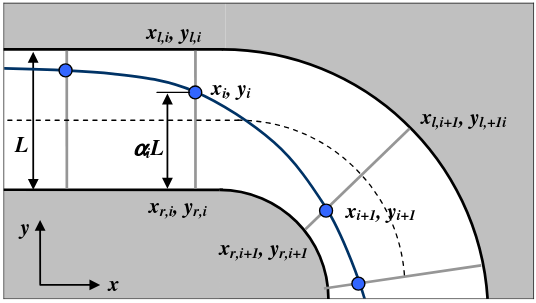
\includegraphics[width=0.65\textwidth]{short-path-expl.png}
	\end{center}
	\caption{}\label{fig:short-path-expl}
\end{figure}

\paragraph{Minima Curvatura}
In questo caso, l'obiettivo è minimizzare la curvatura della raceline, incorporando gli ulteriori vincoli
di orientamento e curvatura descritti precendentemente paragrafo
\hyperref[par:spline-def]{\textit{Definizione di spline}} nel sottocapitolo \ref{sub:formal-def}.\\
Il modello viene definito come:
\[
	\begin{aligned}
		min\ [a_i \dots a_N] & \sum_{i=1}^{N} \kappa_i^2 \\
		subj.\ to\ & M \cdot A = b \\
		& a_i \in [a_{i, min}, a_{i, max}] \quad \forall 1 <= i <= N
	\end{aligned}
\]
dove $\kappa_i$ è la curvatura della funzione in un sample $i$, definita come:
\[
	\kappa_i = \frac{{x'_i} {y''_i} - y'_i x''_i}{({x'_i}^2 + {y'_i}^2)^\frac{3}{2}}
\]
dunque elevando al quadrato:
\[
	\kappa_i^2 = \frac{{x'_i}^2 {y''_i}^2 - 2 x'_i x''_i y'_i y''_i + {y'_i}^2 {x''_i}^2}{({x'_i}^2 + {y'_i}^2)^3}
\]


